\documentclass{article}

% include graph
\usepackage{graphicx}
% if then else
\usepackage{ifthen}
% for sub itermize
\usepackage{outlines}
% using color package
\usepackage[usenames,dvipsnames]{color}
% 用于产生一种数学用的花体字  
\usepackage{mathrsfs}
% 数学符号  
\usepackage{amsmath,amssymb}
% 专门处理数学粗体的bm宏包
\usepackage{bm}
% 高质量数学字体/黑体  
\usepackage[cmintegrals]{newtxmath}
% Expectation by \E
% just use "\mathbb{E}"
% \DeclareMathOperator{\E}{\mathbb{E}}
% 英文花体, e.g., $\mathcal{D}$
%----------------------------- THE ARTICLE -------------------------------

\begin{document}

\begin{titlepage}
    
\includegraphics[height=3.4cm]{../others/sedes.pdf}
    \\ \\
    \textbf{Machien Learning and Inductive Inference [H02C1a]}
    \\ \\ 
    \textbf{Xinhai Zou (r0727971)}
\end{titlepage}

\pagenumbering{roman} 
\tableofcontents
\clearpage
\pagenumbering{arabic}
\setcounter{page}{1}

\section{Lecture 1: Introduction, Version spaces}
\subsection{Some ML examples in practice}
\begin{enumerate}
    \item Autonomous cars
    \item The Robosail project
    \item The Robot Scientist
    \item Infra Watch, "Hoolandse brug" - the bridge
    \item Language learning
    \item Automating manual tasks
\end{enumerate}

\subsection{Machine Learning}
\textbf{Definition} of machine learning: it is the study of how to make programs improve their performance on certain tasks from own (experience).
\\In this case:
\begin{itemize}
    \item "performance" = speed, accuracy
    \item "experience" = earlier observations
\end{itemize}
\textbf{Machine Learning vs. other AI} \\
In \textbf{machine learning}, the key is \textbf{data}, examples of questions and their answer; observations of earlier attempts to solve the problem
\\ In \textbf{inductive inference}, it is reasonsing from \textbf{specific} to \textbf{general}, statistics: sample -> population; from \textbf{concrete observations} -> \textbf{general theory}

\subsection{Machine Learning learning landscape}
\begin{outline}
    \1 tasks
        \2 clustering
        \2 classification
        \2 regression
        \2 reinforcement learning
    \1 techniques
        \2 Convex optimization
        \2 Matrix factorization
        \2 Transfer learning
        \2 Learning theory
        \2 Greedy search
    \1 models
        \2 automata
        \2 neural network
        \2 deep learning
        \2 statistical relational learning
        \2 decision trees
        \2 support vector machines
        \2 nearest neighbors
        \2 rule learners
        \2 bayesian learning
        \2 probabilisitc graphical models
    \1 applications
        \2 natural language processing
        \2 vision
        \2 speech
    \1 related courses
        \2 neural computing
        \2 support vector machine
        \2 uncertainty in AI
        \2 data mining
        \2 genetic algorithms and evolutionary computing
\end{outline}

\subsection{Some basic concepts and terminology}
\begin{outline}
    \1 Predictive learning
        \2 Definition: learn a model that can predict a particular property/ attribute/ variable from inputs
        \2 Binary classification: distinguish instances of class C from other instances
        \2 Classification: assign a class C (from a given set of classes) to an instances
        \2 Regression: assign a numerical value to an instance
        \2 multi-label classification: assign a set of labels (from a given set) to an instance
        \2 multivariate regression: assign a vector of numbers to an instances
        \2 multi-target prediction: assign a vector of values (numerical, categorical) to an instances
    \1 Descriptive learning
        \2 Definition: given a dataset, describe certain patterns in the dataset, or in the population it is drawn from
    \1 Typical tasks in ML
        \2 function learning: learn a function X->Y taht fits the given data
        \2 distribution learning: distribution learning
            \3 parametric: the function family of the distribution is known, we only need to estimate its parameters
            \3 non-parametric: no specific function family assumed
            \3 generative: generate new instances by random sampleing from it
            \3 discriminative: conditional probability distribution
    \1 Explainable AI (XAI)
        \2 Definition: means that the decisions of an AI system can be explained
        \2 Two different levels:
            \3 We understand the (learned) model
            \3 We understand the individual decision
\end{outline}

\subsection{Input formats (predictive learning)}
\begin{outline}
    \1 Set
        \2 training set: a set of examples, instance descriptions that include the target property (a.k.a. labeled instances)
        \2 prediction set: a set of instance descriptions that do not include the target property ('unlabeled' instances)
        \2 prediction task: predict the label of the unlabeled instances
    \1 Outcome of learning process
        \2 transductive learning: the predictions themselves
        \2 inductive learning: a function that can predict the label of any unlabeled instance
    \1 Explainable AI
        \2 interpretable: can be intepred
        \2 black-box: non-interpretable
    \1 Learning
        \2 Supervised learning: from labeled
        \2 Unsupervised learning: from unlabeled
        \2 Semi-supervised learning: from a few labeled and many unlabeled
    \1 Format of input data
        \2 input is often assumed to be a set of instances that are all described using the same variables (features, attributes)
        \2 i.i.d.: independent and identically distributed
            \3 tabular data (NN)
            \3 sequences
            \3 trees
            \3 graph
            \3 raw data: learning meaningful feaures from raw data
            \3 knowledge: inductive logic programming
\end{outline}

\subsection{Output formats, methods (predictive learning)}
The \textbf{output} of a learning system is a model.
\begin{outline}
    \1 output
        \2 parametrized functions
        \2 ocnjunctive concepts: a conjuntive concept is expressed as a set of conditions, all of which must be true
        \2 rule sets (if...then...else...)
        \2 decision trees
        \2 neural networks
        \2 probabilisitc graphical models
    \1 search methods
        \2 discrete spaces - methods: hill-climbing, best-first
        \2 continuous spaces - methods: gradient descent
    \1 typically
        \2 model structure not fixed in advanced - discrete
        \2 fixed model structure, tune numerical parameters - continuous
    \1 hypothesis space
        \2 definition: all possible instances
        \2 for robot example: \{B,R,M,?\} x \{S,T,?\} x \{L,W,?\} x \{1,2,?\}
    \1 Verson space
        \2 using candidate elimination
        \2 pros
            \3 can be used for discrete hypothesis spaces
            \3 search for all solutions, rather than just one, in an efficient manner
            \3 importance of generality ordering
        \2 cons
            \3 not robust to noise
            \3 only conjunctive concepts
\end{outline}
\pagebreak


\section{Lecture 2: Induction of decision tree}
\subsection{Overview of DT}
\begin{outline}
    \1 A decision tree represents a decision procedure where
        \2 you start with one question
        \2 the answer will determine the next question
        \2 and repeat, untill you reach a decision
    \1 We will usually call the questions "tests" and the decision a "prediction"
    \1 attribute
        \2 input attribute X = \{X$_{1}$, X$_{2}$ ..., X$_{n}$\}
        \2 target attribute Y
        \2 the tree represents a function f: X -> Y
    \1 Example: Playing Tennis Tree
        \2 Outlook: X$_{1}$ = \{Sunny, Overcast, Rainy\}
        \2 Humidity: X$_{2}$ = \{High, Normal\}
        \2 Wind: X$_{3}$ = \{Strong, Weak\}
        \2 Tennis: Y = \{Yes, No\}
        \2 The tree represents a function Outlook x Humidity x Wind -> Tennis
    \1 Boolean tree
    \1 Continuous input attributes
        \2 We cannot make a different child node for each possible value!
        \2 Solution: use comparative test -> a finite number of possible outcomes
    \1 Type of trees
        \2 target attribute Y is nomial -> classification tree
        \2 target attribute Y is numerical -> regression tree
    \1 \textbf{Advantages of Tree (Why tree?)}
        \2 Learning and using tree is \textbf{efficient}
        \2 Tend to have \textbf{good predictive accuracy}
        \2 Tree is \textbf{interpretable}
\end{outline}

\subsection{Learn trees from data}
\begin{outline}
    \1 Two tasks for DT
        \2 Task 1: find the smallest tree T such that $\forall$(x,f(x))$\in$D: T(x)=f(x) (meaning that only fullfill current data set)
        \2 Task 2: find the tree T such that for x drawn from population \emph{D}, T(x) is (on average) maximally similar to f(x) (T:model tree from data set D, f(x):true function in population \emph{D})
            \3 loss function: l: Y$_{1}$ x Y$_{2}$ -> R (where Y$_{1}$ is predicted value, Y$_{2}$ is actual value)
            \3 risk R of T, the expectation of loss function, is $E_{x{\sim}D}[l(T(x),f(x))]$, which is needed to be minimal.
    \1 the basic principle
        \2 The approach is known as "Top-down induction of decision trees (TDIDT)", or "recursive partitioning"
            \3 1. start with the full data set D
            \3 2. find a test such that examples in D with the same outcome for the test tend to have the same value of Y
            \3 3. split D into subsets, one for each outcome of that test
            \3 4. repeat this procedure on each subset that is not yet sufficiently "pure" (meaning, not all elements have the same Y)
            \3 5. keep repeating until no further splits possible
    
\end{outline}

\section{Lecture 3: Learning sets of rules}
\subsection{Linear regression}
Decision tree vs. linear regression
\begin{outline}
    \1 "Linear model": $Y = a + b_{1}X_{1} + b_{2}X_{2} + ... + b_{k}X_{k}$
        \2 usually fit such that sum of squared vertical deviations from line is minimal
        \2 what can we learn from such linear model?
            \3 for predicting Y, given Xi
            \3 for understanding how well Y can be predicted from Xi
            \3 for understanding what the effect of each Xi is on Y
            \3 for visualizing the connection between Xi and Y
            \3 the linear correlation r tells us how well the points fit a line $-1 \le r \le 1$
            \3 the coefficient of determination $R^{2}$ tells us to what extent Y is determined by the $X_{i}$, $0 \le R^{2} \le 1$
        \2 careful with interpretation of coefficients
            \3 coefficients are not scale-free
            \3 "multicollinearity": correlations among $X_{i}$
    \1 important assumptions
        \2 effect of each variable on target is constant (does not depend on other variables)
        \2 effect of different variables are cumulative (add up)
    \1 complex terms
        \2 "overall" coefficient of $X_{2}$ is $(b_{2} + b_{12}X_{1})$ effect of $X_{2}$ on $Y$ depends on $X_{1}$
    \1 nominal variables
        \2 for nominal $X_{i}$ with k values, introduce k-1 "0/1" variables, called "indicator" or "dummy" variables <- \textcolor{red}{Question: do not understand the dummy!!!}
\end{outline}

\subsection{Trees vs. linear regression vs. inductive bias}
\begin{outline}
    \1 Each learning approach has a "bias": implicit assumptions it makes.
    \1 Removing all bias?
        \2 bias-free learning is imporssible!
        \2 no single best method for learning!
        \2 for VS, the bias is "it assumes conjunctive concepts". -> without bias, no generalization.
        \2 all of learning models have their own bias = implicit assumptions about what properties the true model has    
    \1 Choices to make
        \2 Modelling your problem as a prediction tasks:
            \3 What is input, what is output (target attribute)?
            \3 Regression, classification, probability prediction?
        \2 Choosing a learning approach
            \3 Efficiency of learning/prediction phase
            \3 Bias (which more fits the problem)
            \3 interpretability of returned models (interpretation)
\end{outline}

\subsection{Rule learning}
Learning sets of classification rules: rule sets:
\begin{enumerate}
    \item "if...then..."
    \item "if...then...else..."
\end{enumerate}
\begin{outline}
    \1 Example: rule sets - define a leap years
        \2 If year is multiple of 400 then leap
        \2 else if year is a multiple of 100 then not leap
        \2 else if year is multiple of 4 then leap
        \2 else not leap
    \1 A decision tree can be turned into a set of rules!
        \2 By learning decision tree to learn rule sets
    \1 principle
        \2 1. High accuracy: when it makes a prediction, it should be correct
        \2 2. Reasonable coverage: it needs not make a prediction for each instance, but the more, the better
    \1 Coule be top-down or bottom-up
        \2 Top-down:
            \3 Start with maximally generally rule
            \3 add literals one by one
            \3 gradually maximize accuracy without sacrificing coverage
        \2 Bottom-up:
            \3 Start with maximally specific rule
            \3 remove literals one by one
            \3 gradually maximize coverage without sacrificing accuracy
\end{outline}
\begin{figure}[htbp]
    \centering
    \includegraphics[height=5cm]{../figs/RS_algorithm.eps}
    \caption{Algorithm for "General algorithm for rule learning"}
    \label{fig:rulesets_algorithm}
\end{figure}

\begin{figure}[htbp]
    \centering
    \includegraphics[height=6cm]{../figs/RSOL_algorithm.eps}
    \caption{Algorithm for "General algorithm for learning one rule"}
    \label{fig:learnonerule_algorithm}
\end{figure}

\begin{outline}
    \1 Top-down: start with an empty rule
    \1 Heuristics for rule learners
        \2 High accuracy (most important), it is not robust to noise
        \2 reasonably high coverage
    \1 if-then-else rules vs. decision lists
        \2 if-then-else rules
            \3 if year is a multiple of 400 then leap
            \3 else if year is a multiple of 100 then not leap
            \3 else if year is multiple of 4 then leap
            \3 else not leap
        \2 decision lists
            \3 if year is a multiple of 400 then leap
            \3 if year is multiple of 4 but not of 100 then leap
        \2 if-then-else rule is more interpretable
        \2 decision list is more compact
        \2 unordered rules vs. ordered rules <- \textcolor{red}{Question: do not understand!!!}
    \1 example-driven top-down rule induction
        \2 works like regular top-down approach, except:
            \3 pick a not-yet-covered example
            \3 consider as hypothesis space, all the rules that cover this example
            \3 search within this hypothesis spaces (much smaller)
        \2 \textbf{pros:} more efficient
        \2 \textbf{cons:} less robust to noise
    \1 other examples: RIPPER, Weka (software)
\end{outline}

\subsection{Association rules}
\begin{table}[htbp]\footnotesize
    \centering
    \caption{Differences with Classification and association rules}
    \begin{tabularx}{\textwidth}{X|X}
    \toprule
    \textbf{Classification rules}&\textbf{Association rules} \\
    \hline
    One target class&Any combinatino of items can be the target \\
    \hline
    Good rules have near 100\% accuracy ("confidence" here)&Rules need not have near 100\% confidence to be interesting \\
    \hline
    Find a minimal set of rules (just enough to classify)&Find a maximal set of rules (all rules that hold) \\
    \bottomrule
    \end{tabularx}
    \label{tab:diff_classification_association_rules}
\end{table}

\begin{outline}
    \1 Overview
        \2 Similar to classification rules, but for descriptive learning instead of predicitve learning
        \2 is to look for the patterns in data
        \2 classification rules are a small subset of association rules?
    \1 General format: if $a_{1}, a_{2}, ..., a_{n}$ then $a_{n+1}, a_{n+2}, ..., a_{n+m}$
    \1 Rule "If <this> then <that>" is charaterized by
        \2 Support: \% of all clients that buy <this>
        \2 Confidence: \% of buyers of <this> that also buy <that>
    \1 Running a classification rule learner clearly will not work well for association rule, since classification rule is only a small subset of association rule
        \2 Solution: APRIORI algorithm
\end{outline}
\pagebreak
\section{Lecture 4: Instance-based learning, Clustering}
\subsection{Instance-based learning}
Basic key idea: just store all training examples
\begin{outline}
    \1 When seeing a new instance:
        \2 Find the most similar cases in the database
        \2 make a prediction based on those instance
    \1 Architypical method: k-nearest-neighbors (k-NN)
        \2 use most frequent class/ mean target among the k nearest neighbors as your prediction
        \2 k is chosen by the user (hyperparameter)
    \1 Similarity
        \2 how close to others, often Euclidean distance for numerical inputs
    \1 Voronoi diagrams
        \2 indicate area where prediction is influenced by same set of examples
        \2 for 1-NN: cell borders are right in the middle between any two data points
        \2 This is called a Voronoi diagram - kNN
    \1 Decision surface
        \2 Decision surface separate regions with different predictions
    \1 Voronoi diagram for k > 1
        \2 To construct diagram for k-NN with k > 1
             \3 Start from diagram for k-1
             \3 for each cell:
                \4 temporarily forget about k-1 nearest neighbors
                \4 split cell according to k'th nearest neighbors
            \3 Merge adjacent cells with same k nearest neighbors
    \1 pros vs. cons
        \2 \textbf{pros}
            \3 "Learning" is very fast - just storing the data
            \3 all detials of the data are kept
        \2 \textbf{cons}
            \3 can be slow at prediction time
            \3 difficulties in high-dimensional spaces
            \3 relies on having a good similarity measure (Euclidean distance - numerical)
            \3 not robust to noise
    \1 for k-NN, large K -> more robust to overfitting? but it is more robust to noise
    \1 difficulties with high-dimensional space - curse of dimensionality - data are distribtued very sparsely in high-D
    \1 Improvement: Different scales
        \2 When dimensions have very differnet scales, Euclidean distance may not work well
            \3 Solution: normalization - normalize all dimensions to comparable scale
            \3 Give irrelevant dimensions a smalelr weight in the Euclidean distance, so they have less influence
            \3 using a closed formula: $w_{i} = 1 - \frac{1}{n} \sum_{k=1}^{c} \sum_{j=1}^{n_{k}} |\bar{x}_{ki} - x_{kji}|$
            \3 with $c$=\#clusters, $n_{k}$=\#elements in cluster k, $x_{ki}$=mean $x_{i}$ in cluster k, $x_{kji}$=$x_{i}$ for j\'th element in cluster k
    \1 Improvenment: distance-werights k-NN
        \2 Why 3-NN, but why not 4-NN
            \3 Solution: no cut-off at k, but have weights gradually decrease with distance
            \3 careful: influence must decrease fast with distance, otherwise faraway cases will dominate the voting (otherwise noise)
    \1 Improvement: locally weighted regression
        \2 for better fitting
            \3 Solution: fit a simple local model
            \3 a linear regression can be okay
    \1 Prototypes
        \2 A prototype is a representattive for a group of instances
        \2 can be an average for elements in a cluster
        \2 note: need to define similarity between instance \& prototype
    \1 Efficient prediction
        \2 Solution: indexing the data helps
\end{outline}

\begin{outline}
    \1 Lazy learners vs. eager learners
        \2 k-NN is called lazy learner
            \3 do not build a model during training, merely store data
            \3 start doing the hard work when asked a question
        \2 eager learners
            \3 generalize before knowing the question
            \3 try to build a global model that will owrk under all circumstances
        \2 lazy learners can use simpler local models - sometime very accurate
            \3 compare: locally weighted linear regression (k-NN) vs. global linear regression
            \3 compare: learn one rule that covers the query instance vs. learn a global rule set
\end{outline}

\subsection{Clustering}
\begin{outline}
    \1 Overview
        \2 Find structure/pattern in the data, in the form of groups of instances that are highly similar to each other
        \2 It is unsupervised machine learning (no labeled samples)
    \1 Find groups (clusters) of instances so that
        \2 instances in the same group are similar
        \2 instances in the difference group are different 
    \1 Definition of clustering
        \2 flat clustering
            \3 returns a partition of the data
        \2 hierarchical clustering
            \3 returns a hierarchy of clusters
    \1 Other definition of clustering
        \2 extensional clustering
            \3 clusters are defined without any description language
        \2 conceptual clustering
            \3 clusters are defiend using a conceptual description language
\end{outline}

\begin{figure}[htbp]
    \centering
    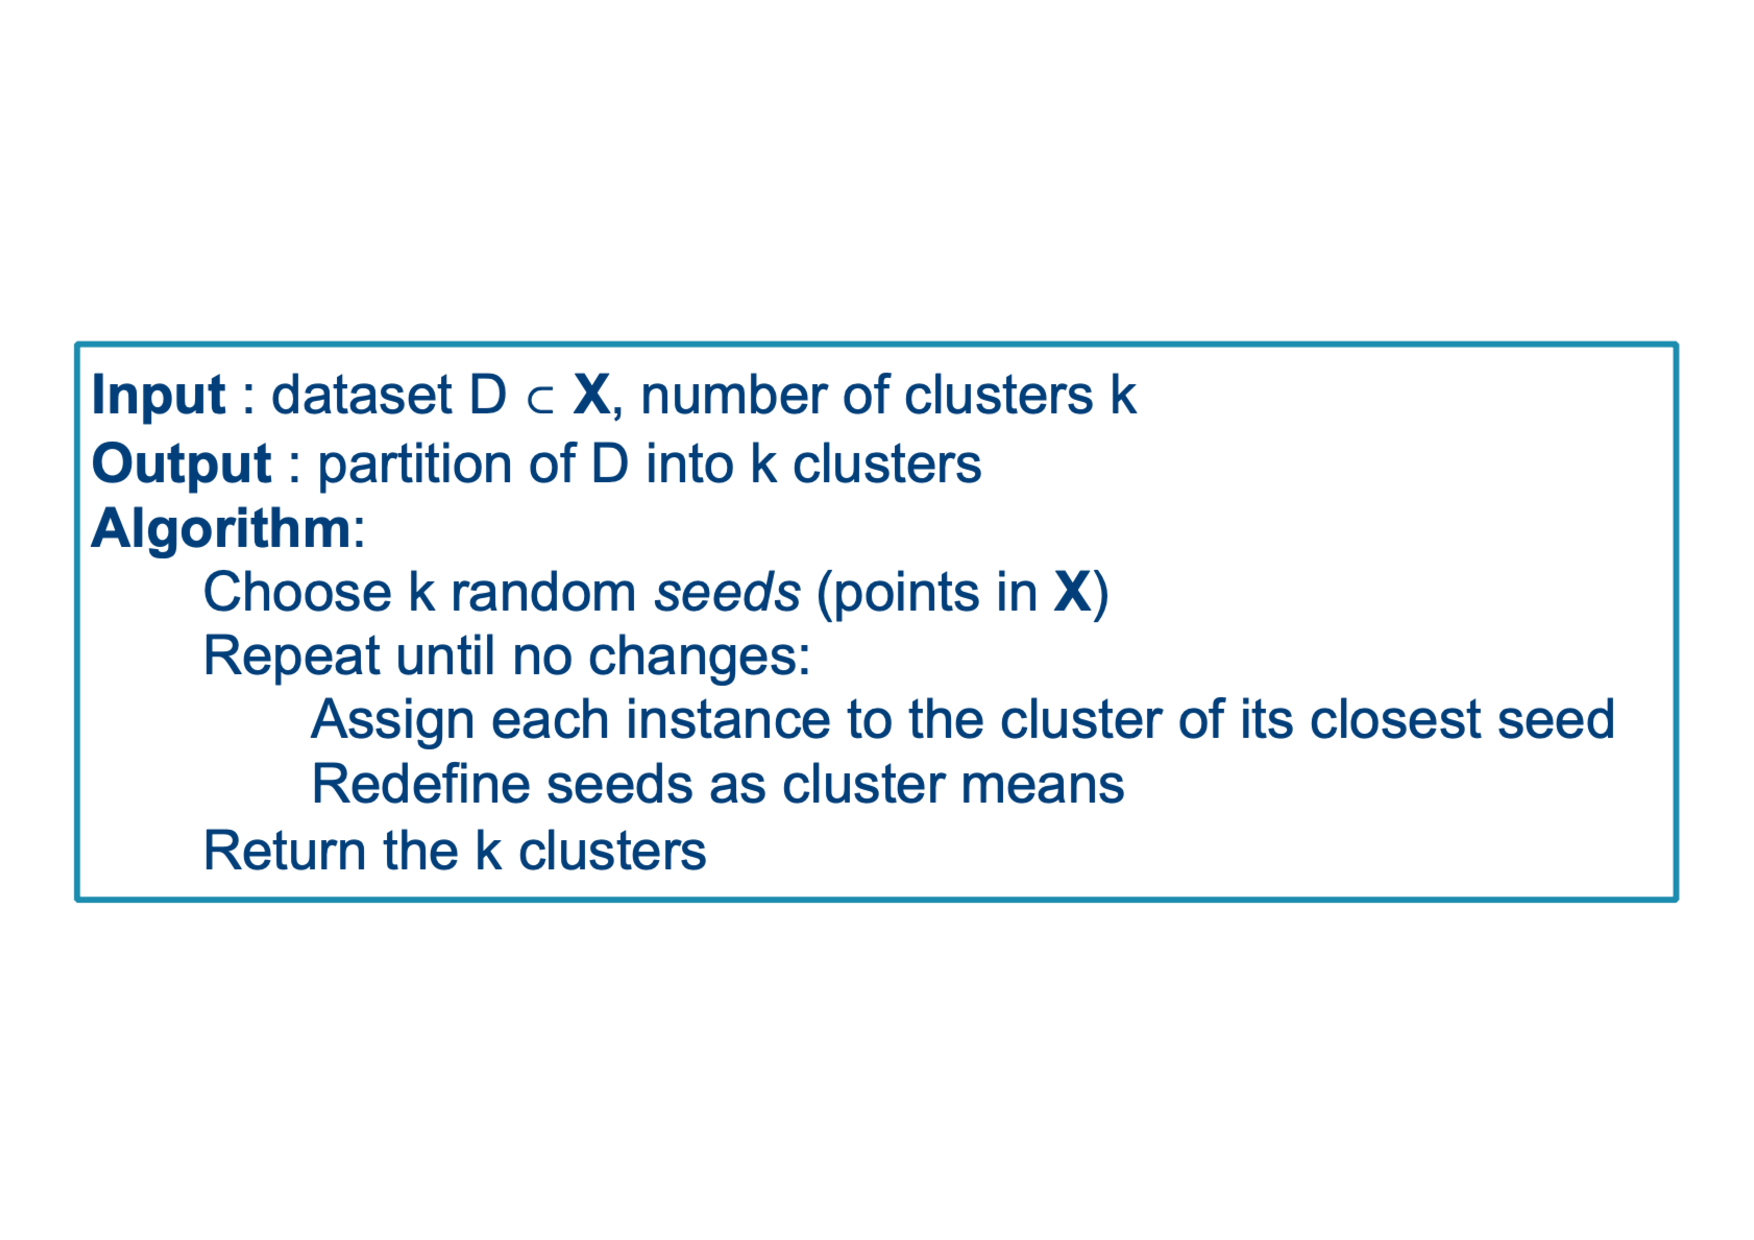
\includegraphics[height=4cm]{../figs/kmean_algorithm.pdf}
    \caption{Algorithm for "Algorithm for flat, extensional clustering: K-means"}
    \label{fig:kmeans_algorithm}
\end{figure}

\begin{outline}
    \1 FLat, extensional clustering
        \2 task: given a set of unlabeled data, find groups of highly similar instances
        \2 some constraints may additionally be given
        \2 procedure: reassign points, recompute seeds, reassign points ..., when no points are re-assigned to another cluster, stop.
    \1 Hierarchical, extensional clustering
        \2 top-down ("divisive") methods
            \3 start with 1 cluster (whole data set)
            \3 divide it into subsets
            \3 subdivide subsets further
        \2 bottom-up ("agglomerative") methods
            \3 start with singleton clusters
            \3 join closest clusters together
            \3 repeat until 1 cluster
    \1 Bottom-up methods
        \2 How does it generalize to distance between clusters? - based on examples
            \3 Single linkage: distance between clusters = distance between each closest point in their cluster
            \3 Complete linkage: distance between clusters = distance between each furthest poin in their clusters
            \3 Average linkage: distance between clusters = distance between average of clusters 
    \1 Conceptual clustering
        \2 Cluster + find a conceptual description of each cluster (in some given description language L)
        \2 Clearly, the clusters are not defined using distance alone! Context is improtant!
    \1 Examples: Cobweb
        \2 Predictability: given cluster, how well can you predict attribute values
        \2 Predictiveness: given attribute values, how well can you predict cluster
        \2 Cobweb is to maximize a combination of both
    \1 Decision tree learning, viewed as clustering
        \2 A decision tree defines a conceptual, hierarchical clustering of the data
            \3 each node = subset of the data
            \3 conceptual description of these data = conjunction of test outcomes from root to node
    \1 Clustering trees
        \2 for regression (original), heuristic minimize average variance of Y within subsets
            \3 $Var(S) = \sum_{(x,y) \in S} \frac{(y - \bar{y})^{2}}{|S|-1|}$ 
            \3 with $\bar{y} = \sum_{(x,y) \in S} \frac{y}{|S|}$
        \2 for clustering (unsupervised clustering tree), given some distance metric d that indicates dissimilarity, we can minimize the average variance of X wihtin subsets
            \3 $Var(S) = \sum_{x \in S} \frac{d(x,\bar{x})^{2}}{|S|-1}$
            \3 with $\bar{x} = \sum_{x \in S} \frac{x}{|S|}$
    \1 Predictive clustering
        \2 overview: it looks like from value -> cluster and from cluster -> value
        \2 Predictive clustering builds a model consisting of 
            \3 a set of clusters
            \3 a function c assigning instances to clusters
            \3 a function p assigning a target value to the instance, given the cluster
        \2 the overall predictive function is then $f(x) = p(c(x),x)$
        \2 the accuracy of f will depend on that of c and p.
            \3 an accurate c requires good predictiveness (from value to cluster)
            \3 an accurate p requires good Predictability (from cluster to value)
\end{outline}

\begin{figure}[htbp]
    \centering
    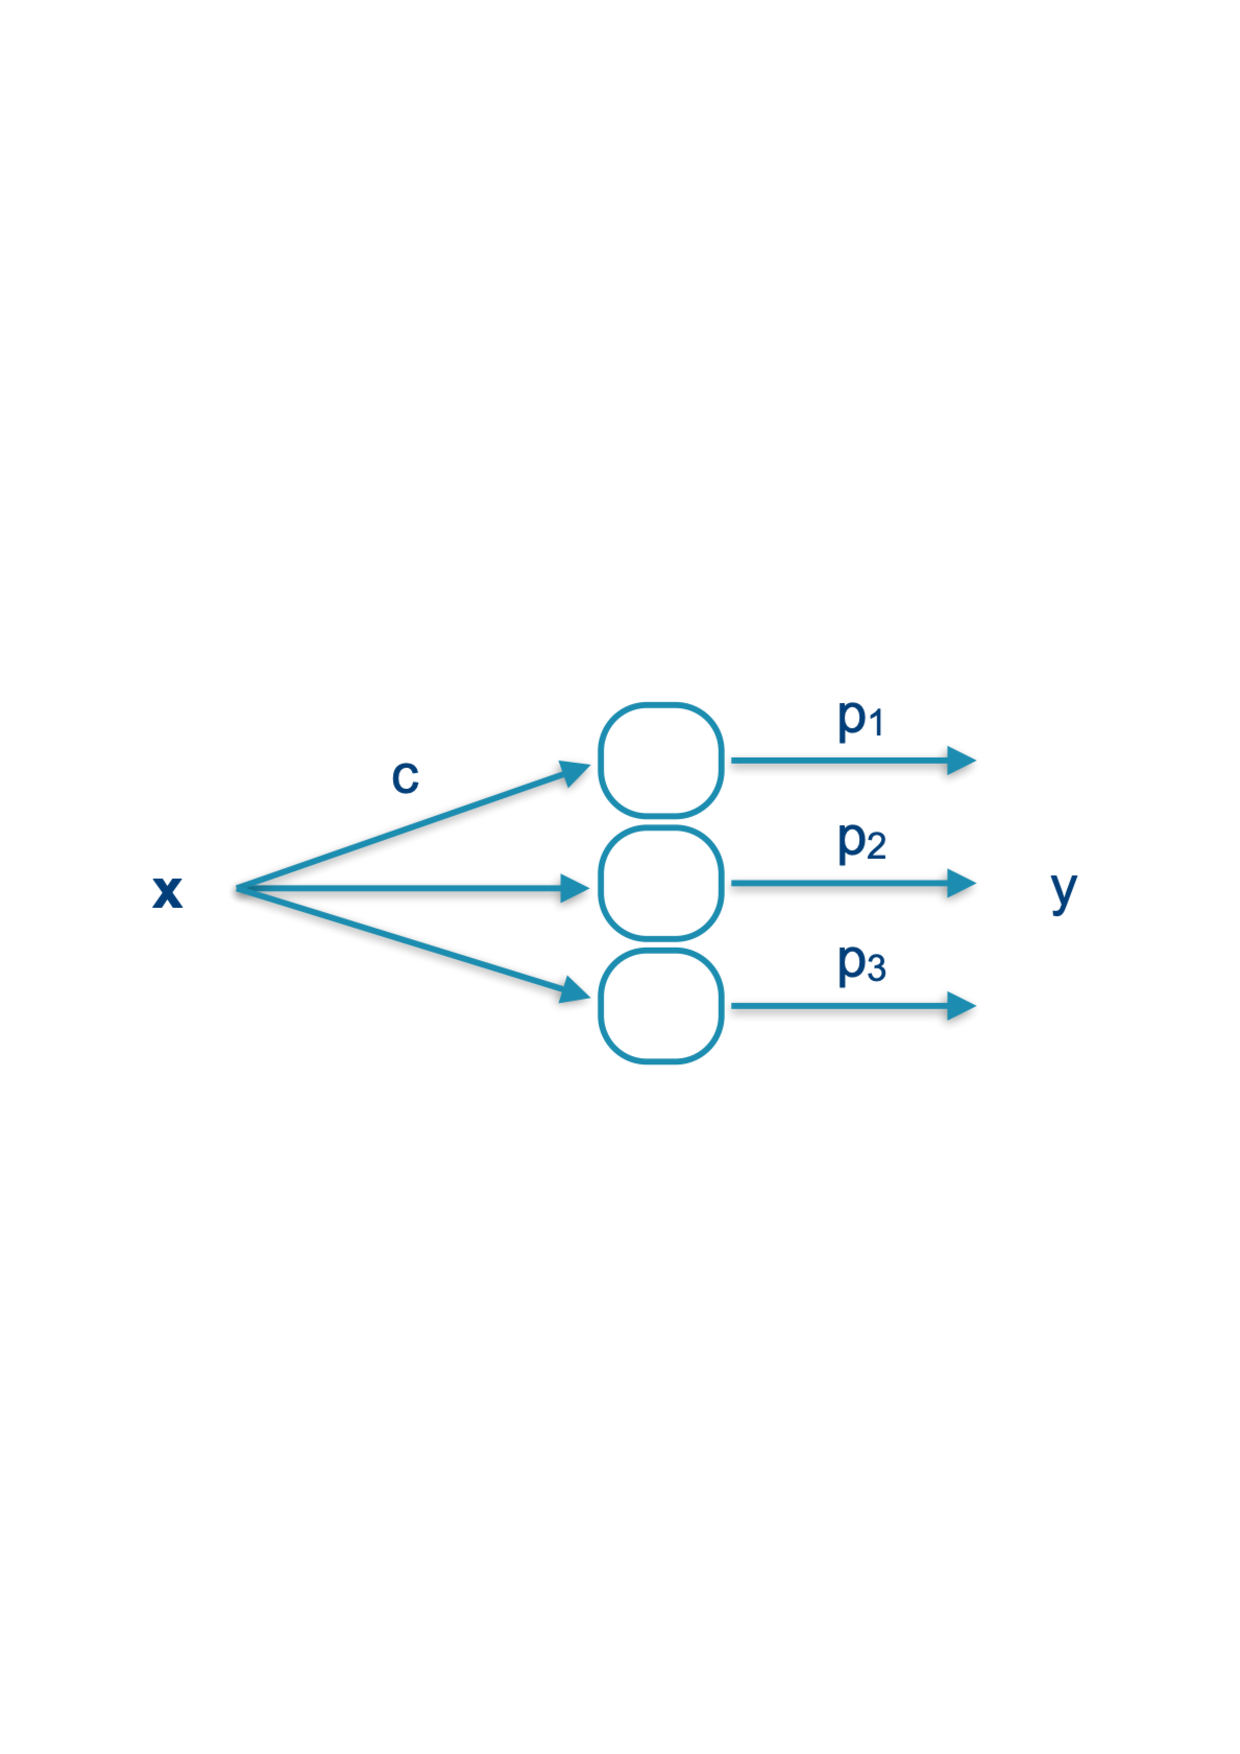
\includegraphics[height=4cm]{../figs/predictive_cluster_scheme.pdf}
    \caption{Algorithm for "Scheme of Predicttive Cluster"}
    \label{fig:scheme_predictive_cluster}
\end{figure}

\begin{outline}
    \1 Similarity measures
        \2 Similarity is often represented using a distance metric
            \3 small distance = high similarity, e.g., euclidean distance, manhattan distance, hamming distance, ...
            \3 $d_{Eucl}(x,x^{\prime}) = \sqrt{\sum_{i} (x_{i}-x_{i}^{\prime})^{2}}$
            \3 $d_{Manh}(x,x^{\prime}) = \sum_{i} |x_{i} - x_{i}^{\prime}|$
        \2 Not all similarity measures can be expressed in that way!
            \3 Distance metric fulfills symmetry and triangle inequality
            \3 Some similarity measures cannot be mapped to such a distance measures
    \1 Learning the similarity measure
        \2 Clustering relies strongly on defining an appropriate similarity measure
        \2 However, this may be very difficult sometime
            \3 Solution: semi-supervised clustering
            \3 Computer learns the similarity from examples of pairs of instances that should be in the same/ in differrent clusters, "must-link" and "cannot-link" constraints
            \3 then start the unlabeled data, (semi-supervised clustering: a few labeled data, many unlabeled data)
    \1 Learning preferred clusterings
        \2 Different clustering algorithms have different biases
            \3 k-means: spherical clusters
            \3 density-based: can return concave clusters
            \3 some methods can even return disconnected cluster
    \1 example of interactive clustering: the COBRAS method
        \2 using an intermediate level of super-instances
            \3 clustering = set of clusters
            \3 cluster = set of super-instances
            \3 super-instance = set of clusters
    \1 Evaluating clusterings
        \2 How can we assess whether a clustering is good or bad?
        \2 explicit objective: minimize intra-cluster variance
        \2 internal criteria: inherent to the clustering
        \2 external criteria: compare to a reference clustering
            \3 rand (random) index
            \3 adjusted rand (random) index (ARI)
\end{outline}
\pagebreak

\section{Lecture 5: Evaluating hypotheses}

\section{Lecture 6: Numerical approaches (ANN, SVM), Computational learning theory}

\section{Lecture 7: Probabilistic approaches, Ensembles}

\section{Lecture 8: Reinforcement learning}

\section{Lecture 9-10: Inductive logic programming}

\clearpage


\end{document}
